%=============================================================================
%
%	Optimization in Banach Spaces
%
%	Continuos evaluation work - Block 1
%
%=============================================================================



%=============================================================================
%	Packages
%=============================================================================

\documentclass[11pt, a4paper]{article}		% document format
\usepackage{graphicx}						% package to insert graphics
\usepackage[english]{babel}
\usepackage[utf8]{inputenc}					% this enables all unicode characters
\usepackage{amsmath, amsfonts, amssymb} 	% maths packages
\usepackage{amsthm}							% theorem styles
\usepackage{fancyhdr}						% package for headers, foot and margin notes
\usepackage{enumitem}						% allows to change the enumeration format in line
\usepackage{tikz}
\usepackage[
  top=2cm,
  bottom=2cm,
  left=3cm,
  right=2cm,
  headheight=17pt, % as per the warning by fancyhdr
  includehead,includefoot,
  heightrounded, % to avoid spurious underfull messages
]{geometry} 




%=============================================================================
%	Commands
%=============================================================================

\providecommand{\U}[1]{\protect\rule{.1in}{.1in}}
\newcommand{\N}{\mathbb{N}}
\newcommand{\E}{\mathcal{E}}
\newcommand{\R}{\mathbb{R}}



%=============================================================================
%	Environment
%=============================================================================

\theoremstyle{plain}
\newtheorem{theorem}{Theorem}%[section]
\newtheorem{lema}[theorem]{Lema}
\newtheorem{exercise}{Exercise}
\newtheorem{algorithm*}{Algorithm}

\theoremstyle{definition}
\newtheorem{solution}{Solution}[exercise]
\renewcommand*{\thesolution}{\theexercise.\alph{solution}}	% Make solution instances enumerate with number of exercise and letter of solution

\usetikzlibrary{calc}



%============================================================================
%	Pagestyle
%=============================================================================

\pagestyle{fancy}		% As we use the fancyhdr pkg need the fancy pagestyle, for more information:
						% http://tug.ctan.org/tex-archive/macros/latex/contrib/fancyhdr/fancyhdr.pdf


%\topmargin 0 pt
%\oddsidemargin 0 pt
%\evensidemargin 0 pt
%\marginparwidth 0 pt


%\textheight 25cm
%\textwidth 400 pt
%\advance\textheight by \topskip

%\parindent 0pt
%\parskip 5mm plus 1mm minus 1mm

\fancyhead[C]{PEC 1}					                	% Central header
\fancyhead[L]{Optimization in Banach Spaces}   				% Left header
\fancyhead[R]{Marc Jovani Bertran}						    % Right header



%=============================================================================
%	Document
%=============================================================================

\begin{document}
	\section*{1}

Resuelva el ejercicio $(2.3)$ de la página 31 del texto base.

\noindent\rule{10cm}{0.4pt}

Consideramos $f$ un funcional cuasi convexo,
entonces para todo $x, y \in S$ definimos $m = \max \{ f(x), f(y) \}$,
tenemos que $x, y \in S_m = \{ p \in S | f(p) \leq m \}$,
y como $f$ es cuasi convexo $S_m$ es un conjunto convexo,
por tanto para todo $\lambda \in [0, 1]$
\begin{equation*}
    \lambda x + (1 - \lambda) y \in S_m \Rightarrow f(\lambda x + (1 - \lambda) y) \leq m = \max \{ f(x), f(y) \}.
\end{equation*}
Como queríamos ver.

Consideramos el funcional $f$ que cumple para todo $x, y \in S$, $\lambda \in [0,1]$
\begin{equation*}
    f(\lambda x + (1 - \lambda) y) \leq \max \{ f(x), f(y) \}.
\end{equation*}
Entonces para cualquier $\alpha \in \R$ veamos que el conjunto $S_\alpha =  \{ p \in S | f(p) \leq \alpha \}$ es convexo.
Para todo $x, y \in S_\alpha$, notemos que $f(x) \leq \alpha$ y $f(y) \leq \alpha$,
y para todo $\lambda \in [0,1]$ tenemos que
\begin{equation*}
    f(\lambda x + (1 - \lambda) y) \leq \max \{ f(x), f(y) \} \leq \alpha,
\end{equation*}
y por tanto $\lambda x + (1 - \lambda) y \in S_\alpha$, implicando que $S_\alpha$ es convexo.

	\section*{2}

Sea $f: S \rightarrow \R$, donde $S$ es un conjunto convexo no vacío de un espacio normado $X$.
Se dice que $f$ es estrictamente cuasi convexa si para todo $x_1 , x_2 \in S$,
con $f(x_1) \neq f(x_2)$, se tiene que
\begin{equation*}
    f(\lambda x_1 + (1 - \lambda) x_2) < \max\{ f(x_1), f(x_2) \}, \; \forall \lambda \in (0, 1).
\end{equation*}

Considérese el problema de optimización dado por:
\begin{equation*}
    \min_{x \in S} f(x).
\end{equation*}

Se pide demostrar el siguiente teorema:

\begin{theorem}
    Supóngase que $f$ es estrictamente cuasi convexa.
    Si en $x_0 \in S$ se alcanza un mínimo local ($x_0$ is a local minimal point),
    entonces en $x_0$ se alcanza, de hecho, un mínimo global ($x_0$ is a global minimal point).
\end{theorem}

\noindent\rule{10cm}{0.4pt}

Siguiendo la misma idea que el Teorema 2.16 del texto base.

Sea $x_0 \in S$ un mínimo local de un funcional estrictamente cuasi convexo $f$.
Entonces $\exists \varepsilon > 0$ tal que $f(x_0) \leq f(x)$ para todo $x \in S \cap B(x_0, \varepsilon)$.

Consideremos un punto $x \in S \setminus B(x_0, \varepsilon)$, tal que $f(x) \neq f(x_0)$.
Definimos $\lambda := \frac{\varepsilon}{\| x_0 - x \|} \in (0, 1)$,
obteniendo $x_\lambda := \lambda x + (1 - \lambda) x_0 \in S$,
\begin{equation*}
    \| x_\lambda - x_0 \| = \| \lambda x + (1 - \lambda) x_0 - x_0 \| = \lambda \| x - x_0 \| = \varepsilon,
\end{equation*}
es decir $x_\lambda \in B(x_0, \varepsilon)$.

Por tanto, utilizando la cuasi convexidad estricta de $f$,
\begin{equation*}
    f(x_0) \leq f(x_\lambda) = f(\lambda x + (1 - \lambda) x_0 - x_0) < \max \{ f(x), f(x_0) \},
\end{equation*}
lo que implica $f(x_0) < f(x)$, por tanto para todo $x \in S$ tenemos que $f(x_0) = f(x)$ o bien $f(x_0) < f(X)$,
asi que $x_0$ es un mínimo global.

	\section*{3}

Se considera en este ejercicio un conjunto $S \subset \R^n$ poliédrico.
Se recuerda que $S$ es poliédrico si se describe como la intersección de un número finito de semiespacios cerrados,
es decir,
\begin{equation*}
    S = \{ x: \langle v_i, x \rangle \leq \alpha_i, \; \forall i = 1, 2, \dots, m \},
\end{equation*}
donde $m \in \N$, $v_i$ es un vector no nulo de $\R^n$ y $\alpha_i$ un escalar,
para todos $i = 1, 2, . . . , m$ (el producto escalar viene denotado por $\langle \cdot, \cdot \rangle$).

De la definición, se deduce que todo conjunto poliédrico es convexo y cerrado.
Indique la demostración.

Por otro lado, se dice que $x \in S$ es un punto extremo de $S$ si $x = \lambda x_1 + (1 - \lambda)x_2$,
con $x_1 , x_2 \in S$ y $\lambda \in (0, 1)$, implica que $x = x_1 = x_2$.
El número de puntos extremos de $S$ es finito.

Se recuerda también que, si $S$ es un conjunto poliédrico compacto,
entonces todo punto $x$ de $S$ se puede expresar como combinación lineal convexa de los puntos extremos de $S$.
Es decir, si $\{ x_1, x_2, \dots, x_r \}$ denota el conjunto de puntos extremos de $S$,
entonces para cada $x \in S$ existen $\lambda_1, \lambda_2, \dots, \lambda_r \geq 0$,
con $\sum_{i = 0}^{r} \lambda_i = 1$ tales que
\begin{equation*}
    x = \sum_{i = 0}^{r} x_i \lambda_i
\end{equation*}

Teniendo en cuenta la teoría anteriormente expuesta, se pide probar el siguiente resultado:
\begin{theorem}\label{ex3_theorem}
    Sea $S$ un conjunto poliédrico compacto no vacío de $\R^n$.
    Considérese el problema
    \begin{equation}\label{ex3_theorem_opt_problem}
        \max_{x \in S} f(x),
    \end{equation}
    con $f: \R^n \rightarrow \R$.
    Si $f$ es cuasi convexa y continua en $S$,
    entonces existe un punto extremo en el que $f$ alcanza un máximo global.
\end{theorem}

\noindent\rule{10cm}{0.4pt}

\begin{lema}\label{ex3_lema_convexity}
    Todo conjunto poliédrico es cerrado y convexo.
\end{lema}

\begin{proof}
    Sea $S$ un conjunto poliédrico.
    Como $S$ es la intersección de conjuntos cerrados es cerrado.

    Los semi-espacios $S_i = \{ x : \langle v_i, x \rangle \leq \alpha_i \}$, que forman $S$, son convexos.
    Para todo $x, y \in S_i$,
    \begin{equation*}
        \langle v_i, \lambda x + (1 - \lambda) y \rangle
        = \lambda \langle v_i, x \rangle + (1 - \lambda) \langle v_i, y \rangle
        \leq \lambda \alpha_i + (1 - \lambda) \alpha_i
        = \alpha_i, \quad \forall \lambda \in [0,1].
    \end{equation*}
    Y la intersección de conjuntos convexos es convexa.
    Por tanto $S$ es convexo.
\end{proof}

Para probar el Teorema \ref{ex3_theorem},
primero vemos que como $S$ es compacto y $f$ es continuo y convexo existe un máximo global.
Consideramos el conjunto de puntos extremos de $S$ y lo denotamos como $E_S$,
sea $\hat{x} \in E_S$ el punto extremo en el que $f$ alcanza un mayor valor,
es decir $f(\hat{x}) \geq x$ para todo $x \in E_S$.
Podemos considerarlo ya que el conjunto $E_S$ es finito.

Sea $S_{f(\hat{x})} = \{ x \in S | f(x) \leq f(\hat(x)) \}$,
notemos que $E_S \subset S_{f(\hat{x})}$,
como $f$ es cuasi convexa $S_{f(\hat{x})}$ es un conjunto convexo.

Supongamos que existe $y \in S$ tal que $y \notin S_{f(\hat{x})}$.
Consideramos la recata $\lambda \hat{x} + (1 - \lambda) y$, para todo $\lambda \in \R$,
esta intersección con $S$ en $\hat{x}$ y en un punto de una cara del poliedro, $x^{(1)}$,
dicha cara es a su vez un poliedro $S^{(1)}$ en una un espacio de dimension menor.
Podemos iterar este proceso eligiendo un punto extremo, $\hat{x}^{(1)}$ del poliedro $S^{(1)}$ y considerando la entre este y $x^{(1)}$,
este proceso es finito ya que la dimension del nuevo poliedro es menor en cada iteración.
\begin{figure}[h!]
\centering
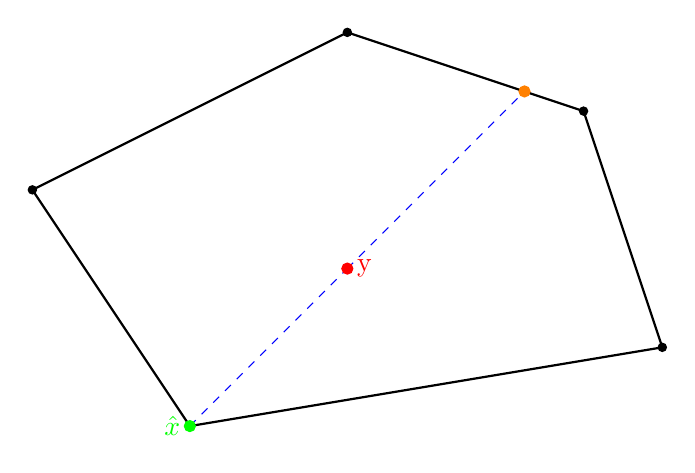
\begin{tikzpicture}

    % Define the vertices of the polyhedron (polygon)
    \coordinate (A) at (0, 0);
    \coordinate (B) at (6, 1);
    \coordinate (C) at (5, 4);
    \coordinate (D) at (2, 5);
    \coordinate (E) at (-2, 3);

    % Draw the polyhedron
    \draw[thick] (A) -- (B) -- (C) -- (D) -- (E) -- cycle;

    % Define the interior point
    \coordinate (P) at (2, 2);

    % Draw a line from one vertex to the interior point
    \draw[dashed, blue] (A) -- (P);

    % Draw a line from the interior point to a point on the boundary
    \draw[dashed, blue] (P) -- ($(D)!0.75!(C)$);

    % Draw the interior point
    \filldraw[red] (P) circle (2pt) node[right] {y};
    
    % Draw the point of contact in the boundary
    \filldraw[orange] ($(D)!0.75!(C)$) circle (2pt);

    % Mark vertices with small circles for clarity
    \filldraw[green] (A) circle (2pt) node[left] {$\hat{x}$};
    \foreach \point in {B, C, D, E}
        \filldraw[black] (\point) circle (1.5pt);

\end{tikzpicture}
\caption{Explicación visual de la demostración}
\label{fig:prove_schema}
\end{figure}

Paramos en cuanto $x^{(l)}$ sea un punto extremo de $S$,
en este caso tenemos que existe $\lambda \in (0,1)$ tal que $x^{(l - 1)} = \lambda x^{(l)} + (1 - \lambda) \hat{x}^{(l - 1)}$,
como $S_{f(\hat{x})}$ es convexo y $x^{(l)}, \hat{x}^{(l - 1)} \in E_S \subset S_{f(\hat{x})}$,
entonces $x^{(l-1)} \in S_{f(\hat{x})}$.
Propagando el razonamiento hacia atrás tenemos que $y \in S_{f(\hat{x})}$.
Que contradice la hipótesis y por tanto $S_{f(\hat{x})} = S$,
que implica que para todo $y \in S$ tenemos que $f(y) \leq f(\hat{x})$,
y por tanto el punto extremo $\hat{x}$ es un máximo global de $f$ en $S$ como queríamos ver.




% \begin{lema}\label{ex3_lema_bounded}
%     Todo conjunto poliédrico compacto esta acotado.
% \end{lema}
% 
% \begin{proof}
%     Sea $S$ un conjunto poliédrico compacto.
%     Para todo $x \in S$ tenemos que
%     \begin{equation*}
%         \| x \| 
%         = \| \sum_{i = 0}^{r} x_i \lambda_i \|
%         \leq \sum_{i = 0}^{r} \lambda_i \| x_i \|
%         \leq \max_{1 \leq i \leq r} \| x_i \|.
%     \end{equation*}
%     Por tanto $S$ esta acotado.
% \end{proof}

% Reformulando el problema (\ref{ex3_theorem_opt_problem}), como,
% \begin{equation}\label{ex3_min_opt_problem}
%     \min_{x \in S} -f(x).
% \end{equation}
% Ambos son equivalentes.
% 
% Por el Lema \ref{ex3_lema_convexity}, es convexo y cerrado,
% y el funcional $f$ es cuasi convexa y continua,
% por tanto $f$ es débilmente semi-continua por debajo.
% Como $S \subset \R^n$ es un sub-espacio de dimension finita,
% Por el Lema \ref{ex3_lema_bounded}$S$ es débilmente secuencialmente semi-compacto,
% como se indica en el Anexo A del texto base.
% 
% Usando el Teorema 2.3 del texto base,
% a su vez por el Lema 2.11 del texto base,
% hemos verificado que existe una solución para el problema (\ref{ex3_min_opt_problem}),
% y por tanto para el problema (\ref{ex3_theorem_opt_problem}).



	\section*{4}

Resuelva el ejercicio (2.8) de la página 31 del texto base.

\noindent\rule{10cm}{0.4pt}

Inspirándonos en la demostración del Teorema 2.23 del texto base,
debemos ver que el nuevo funcional $f$ es quasi convexo y continuo,
ya que el conjunto $S$ no ha cambiado y sigue siendo cerrado, acotado y convexo.
De esta manera resolveríamos el ejercicio aplicando el Teorema 2.12 del texto base.

Veamos que el funcional $f$ es convexo.

Dados $u, v \in S$ y $\lambda \in [0,1]$,
\begin{equation*}
\begin{aligned}
    f(\lambda u + (1 - \lambda) v)
        & = \max_{t \in [t_0, t_1]} \left| x_0 - \hat{x}(t) + \int^{t}_{t_0} e^{A (t - s)} B (\lambda u(s) + (1 - \lambda) v(s)) \right| \\
        & = \max_{t \in [t_0, t_1]} \left| x_0 - \hat{x}(t) + \lambda \int^{t}_{t_0} e^{A (t - s)} B u(s) + (1 - \lambda) \int^{t}_{t_0} e^{A (t - s)} B v(s) \right| \\
        & = \max_{t \in [t_0, t_1]} \left| \lambda \left( x_0 - \hat{x}(t) \int^{t}_{t_0} e^{A (t - s)} B u(s) \right) 
            + (1 - \lambda) \left( x_0 - \hat{x}(t) \int^{t}_{t_0} e^{A (t - s)} B v(s) \right) \right| \\
        & \leq \max_{t \in [t_0, t_1]} \left( \lambda \left| x_0 - \hat{x}(t) \int^{t}_{t_0} e^{A (t - s)} B u(s) \right| 
            + (1 - \lambda) \left| x_0 - \hat{x}(t) \int^{t}_{t_0} e^{A (t - s)} B v(s) \right| \right) \\
        & \leq \lambda \max_{t \in [t_0, t_1]} \left| x_0 - \hat{x}(t) \int^{t}_{t_0} e^{A (t - s)} B u(s) \right| 
            + (1 - \lambda) \max_{t \in [t_0, t_1]} \left| x_0 - \hat{x}(t) \int^{t}_{t_0} e^{A (t - s)} B v(s) \right| \\
        & = \lambda f(u) + (1 - \lambda) f(v),
\end{aligned}   
\end{equation*}
donde hemos usado la desigualdad triangular y el hecho que el máximo de la suma de dos funciones positivas es menor que la suma de sus máximos.

Para ver la continuidad de $f$,
definimos el operador lineal
\begin{equation*}
    Lu(t) = \int^{t}_{t_0} e^{A (t - s)} B u(s) ds,
\end{equation*}
que es acotado y por tanto continuo,
como se muestra en la demostración del Teorema 2.23 del texto base y en un documento proporcionado por la coordinadora de la asignatura.

El valor absoluto es una función continua, por tanto aplicado a otra función continua el resultado sigue siendo una función continua,
con esto tenemos que $| x_0 - \hat{x}(t) + Lu(t) |$ es continuo.

Finalmente como $L$ es continuo en un conjunto compacto es también uniformemente continuo con respecto a $t$,
por tanto el máximo respecto a $t$ de la function $| x_0 - \hat{x}(t) + Lu(t) |$ es continuo,
resultando en que $f$ es continuo.



\end{document}